\documentclass[aspectratio=169]{beamer}

\usepackage[utf8]{inputenc}
\usepackage[T1]{fontenc}
\usepackage[spanish,es-tabla]{babel}
\usepackage{lmodern}
\usepackage{graphicx}
\usepackage{booktabs}
\usepackage{hyperref}
\usepackage{xcolor}

\usetheme{Madrid}
\usecolortheme{default}
\setbeamertemplate{navigation symbols}{}
\setbeamertemplate{footline}[frame number]

\definecolor{TitleBlue}{RGB}{23,50,77}
\definecolor{SoftBlue}{RGB}{234,241,248}

\setbeamercolor{title}{fg=TitleBlue}
\setbeamercolor{frametitle}{fg=TitleBlue}
\setbeamercolor{structure}{fg=TitleBlue}
\setbeamercolor{block title}{fg=TitleBlue,bg=SoftBlue}
\setbeamercolor{block body}{bg=white}

\title{Sistema LLM para análisis financiero histórico\\mediante generación automática de código}
\author{Carlos Ruiz Oyarzun}
\institute{Trabajo Fin de Máster}
\date{2026}

\begin{document}

\begin{frame}
  \titlepage
\end{frame}

\begin{frame}{Idea y motivación}
La idea del trabajo surge de una pregunta sencilla: si un LLM ya puede interpretar consultas y generar código, ¿hasta qué punto se puede usar para ayudar a una persona a interpretar mejor datos históricos de la bolsa?

\vspace{0.4cm}

La motivación no era aceptar una respuesta de caja negra, sino construir un flujo que:
\begin{itemize}
  \item deje artefactos intermedios revisables;
  \item haga visibles los datos usados y los cálculos ejecutados;
  \item permita localizar el punto de fallo cuando algo sale mal.
\end{itemize}

\vspace{0.2cm}
Por eso el objetivo no es construir un asesor financiero ni un sistema de predicción, sino una herramienta de apoyo más explicativa, trazable y controlada.
\end{frame}

\begin{frame}{Pequeña revisión del estado del arte}
\begin{itemize}
  \item El ámbito financiero tiene particularidades propias, como muestran modelos especializados como FinBERT o BloombergGPT.
  \item Las arquitecturas con agentes permiten separar tareas y combinar el modelo con herramientas externas.
  \item La generación de código permite apoyar la respuesta en cálculos observables, no solo en texto plausible.
\end{itemize}

\vspace{0.3cm}
La propuesta se sitúa precisamente ahí: usar un modelo generalista dentro de un flujo fijo, con validaciones, ejecución controlada y trazabilidad.
\end{frame}

\begin{frame}{Visión general del sistema}
Esta diapositiva corresponde a la visión general del sistema desarrollada en el apartado 5.1 de la memoria.

\vspace{0.4cm}

\begin{center}
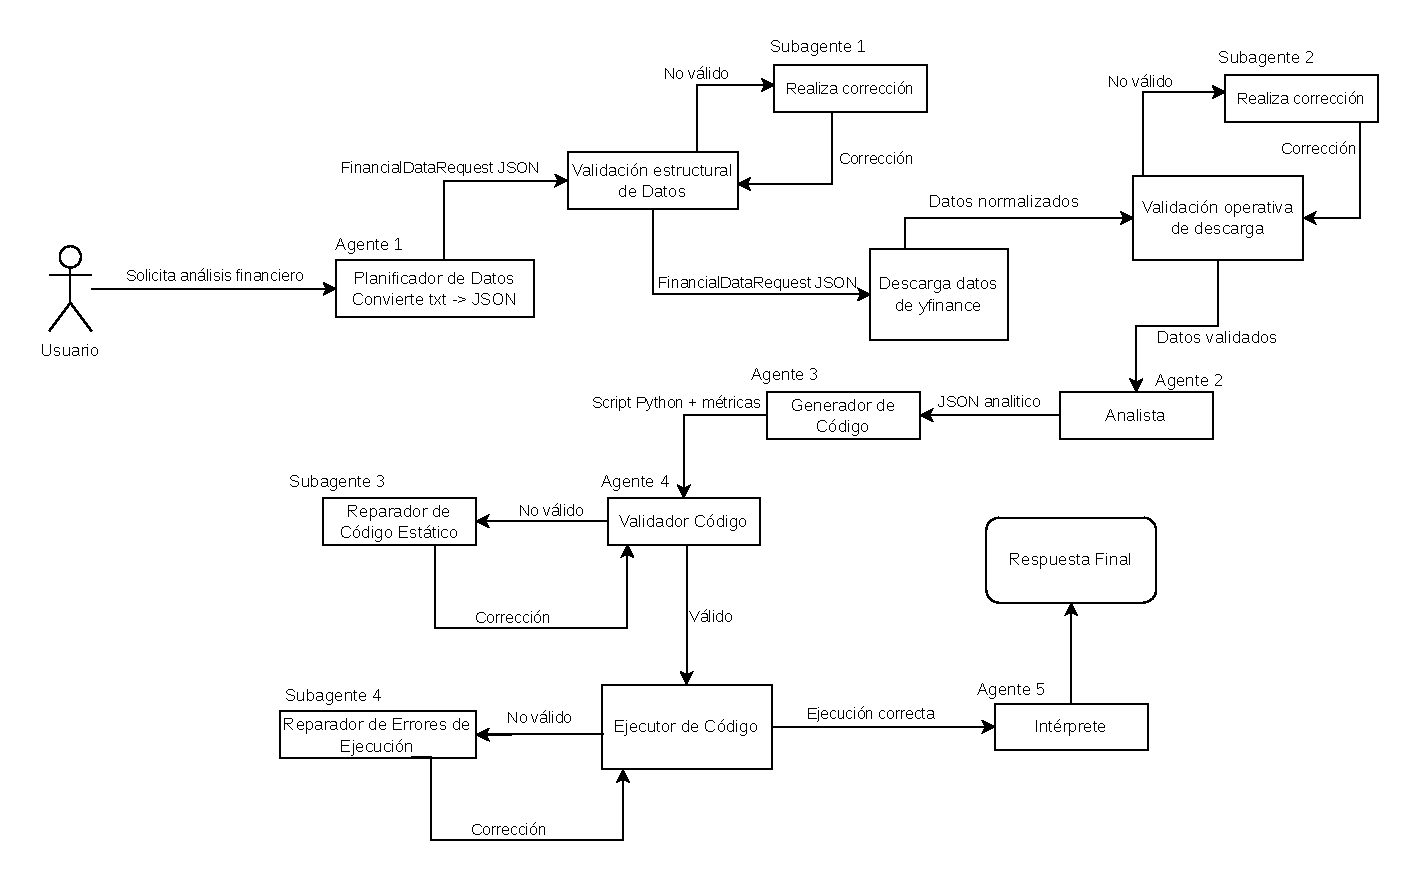
\includegraphics[width=0.92\textwidth,page=1]{FlujoNuevo5.drawio.pdf}
\end{center}

\vspace{0.2cm}
Aquí solo interesa mostrar el recorrido completo de una consulta. En la siguiente diapositiva se explica con más detalle qué ocurre en cada fase.
\end{frame}

\begin{frame}{Flujo de ejecución por fases}
\begin{columns}[T]
\column{0.47\textwidth}
\begin{block}{Fases}
\begin{enumerate}
  \item Resolución y validación de datos.
  \item Planificación analítica.
  \item Generación de código.
  \item Validación y ejecución.
  \item Interpretación final.
\end{enumerate}
\end{block}

\column{0.47\textwidth}
\begin{block}{Qué aporta el flujo}
\begin{itemize}
  \item Base de datos real y validada.
  \item Plan analítico explícito.
  \item Código ejecutable en lugar de solo texto.
  \item Validación previa y comprobación de runtime.
  \item Respuesta final apoyada en resultados observables.
\end{itemize}
\end{block}
\end{columns}

\vspace{0.2cm}
Si una fase falla, se activan rutas de reparación específicas y acotadas.
\end{frame}

\begin{frame}{Ejemplo completo de ejecución}
\textbf{Consulta elegida:}

\vspace{0.2cm}

\begin{quote}
Analiza AAPL en 3 meses y explica qué se puede concluir solo con estos datos históricos.
\end{quote}

\vspace{0.3cm}

En lugar de recorrer todas las trazas, se muestran tres artefactos representativos:
\begin{itemize}
  \item salida del Agente 1 en la fase de datos;
  \item fragmento del Agente 3 en la fase de código;
  \item respuesta final del Agente 5.
\end{itemize}
\end{frame}

\begin{frame}[fragile]{Ejemplo completo: Agente 1}
\textbf{Salida estructurada del \texttt{FinancialDataRequest}}

\begin{verbatim}
{
  "provider": "yfinance",
  "instruments": [{"ticker": "AAPL"}],
  "interval": "1d",
  "period": "3mo",
  "required_fields": [
    "Open", "High", "Low",
    "Close", "Adj Close", "Volume"
  ]
}
\end{verbatim}

La consulta deja de ser texto libre y se convierte en un contrato de datos formal y validable.
\end{frame}

\begin{frame}[fragile]{Ejemplo completo: Agente 3}
\textbf{Fragmento representativo del código generado}

\begin{verbatim}
payload = json.loads(Path(sys.argv[1]).read_text())
tickers = payload.get("tickers", [])
csv_paths = payload.get("csv_paths", [])

close = load_close_prices(csv_paths, tickers)
data = load_market_data(csv_paths, tickers)

ret_3mo = (close_series.iloc[-1] - close_series.iloc[0]) / close_series.iloc[0]
vol_3mo = close_series.pct_change().std()
\end{verbatim}

Aquí el análisis deja de ser una descripción abstracta y se convierte en código ejecutable.
\end{frame}

\begin{frame}[fragile]{Ejemplo completo: Agente 5}
\textbf{Respuesta final legible para el usuario}

\begin{verbatim}
Análisis de AAPL (últimos 3 meses)

- Precio de cierre promedio: 278.00
- Máximo: 315.20
- Mínimo: 246.63
- Retorno total: 16.40 %
- Volatilidad diaria: 1.45 %
- Drawdown máximo: -7.82 %
\end{verbatim}

La respuesta visible es la última capa de un proceso previo de datos, planificación, código, validación y ejecución.
\end{frame}

\begin{frame}{Manera en que se evalúa el proyecto}
\begin{itemize}
  \item Batería de 50 consultas financieras organizada en tres niveles de complejidad: A, B y C.
  \item La unidad de análisis es la consulta completa de extremo a extremo.
  \item Un caso solo se considera completado si el flujo produce una respuesta final utilizable.
  \item Los casos completados se revisan con una rúbrica de cinco criterios.
\end{itemize}

\vspace{0.2cm}

\begin{block}{Criterios cualitativos}
Adecuación a la consulta, cobertura analítica, coherencia, claridad y prudencia.
\end{block}
\end{frame}

\begin{frame}{Resultados}
\begin{table}
\centering
\small
\begin{tabular}{lrrrr}
\toprule
Nivel & Casos & Completados & No completados & Tasa \\
\midrule
A & 10 & 8 & 2 & 80\% \\
B & 20 & 12 & 8 & 60\% \\
C & 20 & 7 & 13 & 35\% \\
\bottomrule
\end{tabular}
\end{table}

\vspace{0.3cm}

\begin{itemize}
  \item 27 de 50 casos completados.
  \item 54\% de completitud global.
  \item La dificultad creciente tensiona sobre todo las fases previas del workflow.
  \item Cuando el sistema completa una consulta, la calidad final suele ser buena.
\end{itemize}
\end{frame}

\begin{frame}{Limitaciones}
\begin{itemize}
  \item La evaluación se realiza con una configuración concreta del sistema y un único modelo.
  \item El flujo depende de un proveedor de datos históricos.
  \item La revisión cualitativa de los casos completados ha sido realizada por el autor.
  \item El alcance del trabajo se limita al análisis histórico.
\end{itemize}
\end{frame}

\begin{frame}{Conclusiones}
\begin{itemize}
  \item La principal aportación es una arquitectura multiagente más trazable, explicable y controlada que una respuesta generativa directa.
  \item Cuando el sistema completa un caso, la calidad final suele ser razonable.
  \item El valor del sistema no está solo en responder, sino en ayudar a explicar mejor lo que muestran los datos.
\end{itemize}
\end{frame}

\end{document}
